
\chapter{Contextualization}

The LHC accelerates two particle beams in opposite directions, where they collide at the detectors. From this head-on collision between two particles results a limited chain reaction of decaying particles, where the detector records most of the final particles. The ATLAS detector can record only some of the characteristics of these particles. A schematic representation of the head-on collision is presented in figure \ref{fig:ttbar}, and it is known as the ttbar system. The particles detected are the bottom quarks (which are detected as a jet of particles) and leptons (electron and muon), while the neutrinos do not react with the detector. In order to reconstruct the collision, the characteristics of the neutrinos must be determined. Since this system obeys a set of properties, related to the calibrated model expected from the collision, it is possible to analytically determine the neutrinos characteristics and reconstruct the event (kinematical reconstruction), and then calculate the degree of certainty associated with the reconstruction.

\begin{figure}[!htp]
	\begin{center}
		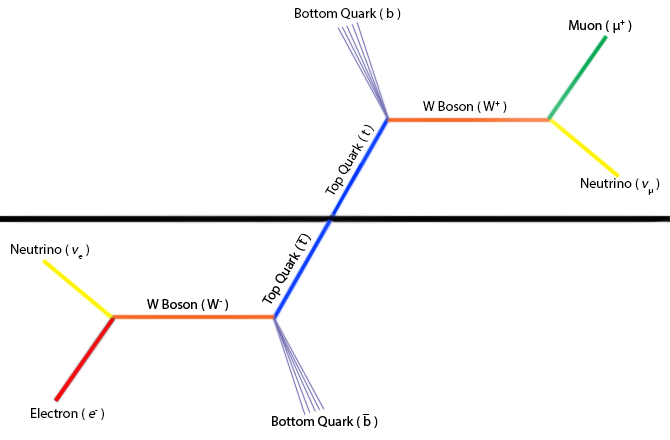
\includegraphics[scale=0.5]{../../common/img/ttbar.png}
		\caption{Schematic representation of the ttbar system.}
		\label{fig:ttbar}
	\end{center}
\end{figure}

During a collision, several particles, bottom quark jets and leptons, are detected. The amount detected can vary from between events, but it is needed at least 2 jets and 2 leptons to reconstruct the ttbar system, as represented in the figure~\ref{fig:ttbar}, but can reach up to 14. However, some of the jets/leptons may not belong to the ttbar system, so it is needed to choose the ones that reconstruct the system with the most accuracy.

By performing the kinematical reconstruction to each combination of all the bottom quark jets and leptons, two by two, and calculating the probability associated with the reconstruction, it is possible to chose only the combination that results on the most accurate reconstruction.

Another factor that can affect the accuracy of the reconstruction is the experimental resolution associated with the ATLAS detector. The detected values for the particles (bottom quark jets and leptons) characteristics are not 100\% accurate. In fact, the measurements made by ATLAS can have a 2\% inaccuracy to the real values. Since these particles are used in the kinematical reconstruction, its accuracy can be affected. To improve the accuracy of these reconstructions, the experimental resolution must be compensated. This can be achieved by varying the values of the bottom quark jets and leptons characteristics, such as the mass or momentum, and use them in the kinematical reconstruction. However, this cannot be performed only once; the search space must be covered a certain amount of times in order to get higher probability of finding a great reconstruction. This means running the kinematical reconstruction as many times as possible, per event, with inputs with different variations.

The execution time of the analysis is very important because of the large amounts of data (events) that must be processed. Since for each event is necessary to reconstruct all the bottom quark jets and leptons combinations, and for each combination a variation is applied a given amount of times, the number of kinematical reconstructions per event can rise quickly, increasing the overall time that takes to process it. A balance between the required quality of the reconstruction, which is directly related to the number of times that the kinematical reconstruction is performed, and the time that takes to process an event must be achieved. 

In the ttH\_dilep analysis, the importance of the kinematical reconstruction (dilep) is even greater. This analysis takes into account the two jets that result from the Higgs boson decay and also tries to reconstruct it. Figure~\ref{fig:ttbarhiggs} schematically represents the ttbar system with the Higgs boson decay and respective jets. After performing the ttbar system reconstruction, i.e., the kinematical reconstruction, and considering the jets used in its best reconstruction, the application uses the remaining jets to reconstruct the Higgs boson. If an event ttbar system is badly reconstructed, the Higgs boson reconstruction will not be accurate. Now, the best final reconstruction is given by the probability of the best kinematical reconstruction and the probability of the respective Higgs boson reconstruction. 

\begin{figure}[!htp]
	\begin{center}
		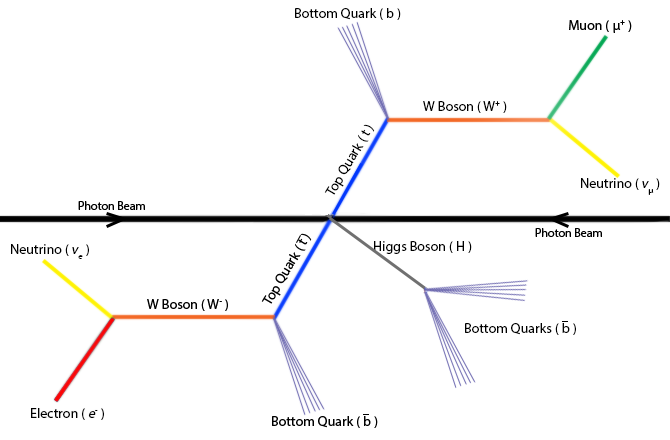
\includegraphics[scale=0.5]{../../common/img/ttbar_higgs.png}
		\caption{Schematic representation of the ttbar system with the Higgs boson decay.}
		\label{fig:ttbarhiggs}
	\end{center}
\end{figure}

By increasing the kinematical reconstruction performance it is possible to perform more reconstructions per event, leading to better and more accurate results. However, it is not possible to narrow the scope of this dissertation work only to the reconstruction; to get the most efficiency from it, it is necessary to consider the jet combination, variance appliance and Higgs reconstruction as other important tasks to improve, and eventually re-design the workflow of this section of the application. The LIP research group has a big interest on improving the kinematical reconstruction, as well as the overall ttH\_dilep analysis, performance, as it would give them an advantage over the other research groups.

\newpage
